
\documentclass{standalone}

\usepackage[T1]{fontenc}
\usepackage{amsmath,amssymb,mathtools}
\newcommand{\set}[1]{\left\{ #1 \right \}}

\usepackage{graphicx}
\definecolor{navyblue}{RGB}{0,0,128}

\begin{document}

\tikzset{cross/.style={cross out, draw=red, thick, minimum size=1.5em, inner sep=0pt, outer sep=0pt},
%default radius will be 1pt. 
cross/.default={1pt}}



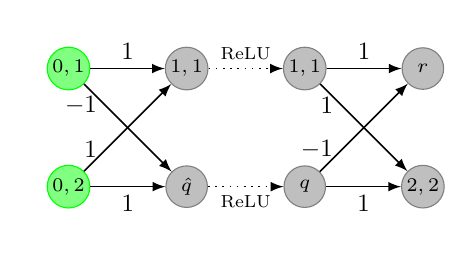
\begin{tikzpicture}[node distance=3cm, font=\scriptsize,auto,
  neuron/.style={circle, inner sep=0.03cm}]

  \node [label=left:{},fill=green!50!white,draw=green,neuron] (1)
  {$\out{0,1}$};

  \node [label=left:{},below of=1,yshift=1.5cm,
  fill=green!50!white,draw=green,neuron] (2) {$\out{0,2}$};

  \node [label=above:{},right of=1, xshift=-1.5cm,
  fill=gray!50!white,draw=gray,neuron] (3) {$\pre{1,1}$};

  \node [label=below:{},minimum size=1.5em, below of=3,yshift=1.5cm,
  fill=gray!50!white,draw=gray,neuron] (4) {$\hat{q}$};

  \node [label=above:{},right of=3, xshift=-1.5cm,
  fill=gray!50!white,draw=gray,neuron] (3b) {$\out{1,1}$};

  \node [label=below:{},minimum size=1.5em,below of=3b,yshift=1.5cm,
  fill=gray!50!white,draw=gray,neuron] (4b) {$q$};


  \node [label=above:{},right of=3b, minimum size=1.5em, xshift=-1.5cm,
  fill=gray!50!white,draw=gray,neuron] (5) {$r$};

  \node [label=below:{},below of=5,yshift=1.5cm,
  fill=gray!50!white,draw=gray,neuron] (6) {$\out{2,2}$};



  % \node [label=right:{$[-1,2]$},yshift=8em,below of=1,right of
  % =1,fill=gray!50!white,draw=gray,circle] (2)
  % {$\out{0,2}$};


  % \node [label=left:{$[-1,1]$},yshift=8em,below of=2,left
  % of=2,fill=gray!50!white,draw=gray,circle] (3)
  % {$\out{0,2}$};


  

  \path[-latex,semithick,every node/.style={->,font=\sffamily\normalsize, scale=0.9}]
  (1) edge node [above] {$1$} (3)
  (1) edge node [near start,left] {$-1$} (4)
  (2) edge node [near start,left] {$1$} (3)
  (2) edge node [below] {$1$} (4)
  (3) edge[dotted] node[font=\scriptsize] [above] {ReLU} (3b)
  (4) edge[dotted] node[font=\scriptsize] [below] {ReLU} (4b)
  (3b) edge node [above] {$1$} (5)
  (3b) edge node [near start,left] {$1$} (6)
  (4b) edge[] node [near start,left,color=black] {$-1$} (5)
  (4b) edge node [below] {$1$} (6);


  %\draw (5.85,-1.7) node[cross, rotate=0] {};

  %\node
  %[neuron,draw,xshift=7cm, minimum size=1.5em,yshift=0.2cm,draw=black,fill=black,text=white]
  %(1) {$q$}
  %child {node [neuron,minimum size=1.5em,draw=black,fill=black,text=white,yshift=0.3cm]
  %(2) {$r$} 
    %child {node [yshift=0.2cm] (4) {} edge from parent[dotted,thick]}
    %child {node [yshift=0.2cm] (5) {} edge from parent[dotted,thick]}}
  %child {node
	  %[neuron,draw,minimum size=1.5em,draw=black,fill=black,text=white,yshift=0.3cm] (3)
  %{$r$} 
    %child {node [yshift=0.2cm] (6) {} edge from parent[dotted,thick]}
    %child {node [yshift=0.2cm] (7) {} edge from parent[dotted,thick]}};
  %\path (1) -- (2) node [midway,left,xshift=-0em,yshift=0em] {$\it{inactive}$};
  %\path (1) -- (3) node [midway,right,xshift=-0em,yshift=0em] {$\it{active}$};
  %\path (2) -- (5) node [midway,right,xshift=-2em,yshift=-1em] {$\it{active}$};
  %\path (3) -- (6) node [midway,left,xshift=2.5em,yshift=-1em] {$\it{inactive}$};
  %\path (3) -- (7) node [midway,right,xshift=0.5em,yshift=-1em]
  %{$\it{active}$};


\end{tikzpicture}

\end{document}
